\documentclass[10pt,letterpaper]{article}
\usepackage[margin=0.6in]{geometry}
\usepackage{graphicx}
\usepackage{booktabs}
\usepackage{enumitem}
\usepackage{hyperref}
\usepackage{xcolor}
\usepackage{listings}
\usepackage{amsmath}
\usepackage{tikz}
\usetikzlibrary{shapes,arrows,positioning,fit,backgrounds}
\usepackage{titlesec}
\usepackage{float}
\usepackage{subcaption}
\titlespacing*{\section}{0pt}{6pt}{2pt}
\titlespacing*{\subsection}{0pt}{4pt}{2pt}
\titlespacing*{\subsubsection}{0pt}{3pt}{1pt}
\setlength{\parskip}{1pt}
\setlength{\floatsep}{4pt}
\setlength{\textfloatsep}{4pt}
\setlength{\intextsep}{4pt}

\definecolor{codegreen}{rgb}{0,0.6,0}
\definecolor{codegray}{rgb}{0.5,0.5,0.5}
\definecolor{codepurple}{rgb}{0.58,0,0.82}
\definecolor{backcolour}{rgb}{0.95,0.95,0.92}

\lstdefinestyle{mystyle}{
    backgroundcolor=\color{backcolour},
    commentstyle=\color{codegreen},
    keywordstyle=\color{magenta},
    stringstyle=\color{codepurple},
    basicstyle=\ttfamily\scriptsize,
    breakatwhitespace=false,
    breaklines=true,
    captionpos=b,
    keepspaces=true,
    showspaces=false,
    showstringspaces=false,
    showtabs=false,
    tabsize=2,
    aboveskip=3pt,
    belowskip=3pt
}
\lstset{style=mystyle}

\hypersetup{
    colorlinks=true,
    linkcolor=blue,
    filecolor=magenta,
    urlcolor=blue,
    citecolor=blue
}

\title{\textbf{Adaptive RDMA Optimization for Distributed LLM Workloads}\\[0.5em]
\large Week 1: Project Overview \& Hardware Setup}
\author{Nathan Gopee\\
MS Computer Science, SUNY New Paltz\\
\texttt{gopeen1@newpaltz.edu}\\[1em]
\small Advisors: Dr. Wafi Danesh \& Dr. Ashley Suchy}
\date{January 2026}

\begin{document}

\maketitle

\section{Overview}

Since I started researching RDMA and LLMs across different hardware setups, I've been comparing vLLM, Ollama, and TensorRT-LLM. Recent patches address a lot of what I'm exploring, but nothing targets RDMA optimizations specifically yet. That's where Soft-RoCE or other RDMA-over-Ethernet solutions come in. I've confirmed it's possible, but debugging and patching will take time. I'm still deciding whether to patch an existing framework or build my own inference framework; each approach has tradeoffs.

\section{Resources}

\subsection{RDMA and InfiniBand Fundamentals}
\begin{itemize}[noitemsep]
    \item \href{https://wiki.archlinux.org/title/InfiniBand}{Arch Wiki: InfiniBand}
    \item \href{https://github.com/teslamotors/ttpoe}{Tesla's TTPoe} -- Tesla's RDMA implementation with optimizations from their xAI cluster
\end{itemize}

\subsection{vLLM and Inference Frameworks}
\begin{itemize}[noitemsep]
    \item \href{https://blog.vllm.ai/2025/09/05/anatomy-of-vllm.html}{Anatomy of vLLM}
    \item \href{https://discuss.vllm.ai/t/vllm-benchmarking-why-is-gpudirect-rdma-not-outperforming-standard-rdma-in-a-pipeline-parallel-setup/1377}{GPUDirect RDMA vs Standard RDMA Benchmarking}
    \item \href{https://www.reddit.com/r/LocalLLaMA/comments/1oyawkl/why_is_vllm_outperforming_tensorrtllm_nvidias/}{vLLM vs TensorRT-LLM Performance Discussion}
\end{itemize}

\subsection{Video Resources}
\begin{itemize}[noitemsep]
    \item \href{https://youtu.be/6t041Lr5FCY}{Distributed LLM Inference Overview}
    \item \href{https://youtu.be/qzNX3ZBPJUA}{RDMA Network Configuration Deep Dive}
    \item \href{https://youtu.be/H1mTv8jI0SE}{GPU Cluster Interconnect Optimization}
    \item \href{https://youtu.be/4l4UWZGxvoc}{Thunderbolt RDMA for Mac Clusters} -- Apple released RDMA over Thunderbolt, which I've been trying to get working on the iMacs for a few semesters
    \item \href{https://www.reddit.com/r/LocalLLaMA/comments/1pq5k6e/jake_formerly_of_ltt_demonstrates_exos/}{Jake's Exo Distributed Inference Demo}
    \item \href{https://youtu.be/nKz92Yr09q8}{InfiniBand Hardware Setup Walkthrough}
    \item \href{https://youtu.be/c3v6R0IbnYs}{vLLM Performance Tuning}
    \item \href{https://youtu.be/L1NPFFRTzLo}{Multi-Node LLM Training Architecture}
\end{itemize}

\section{Hardware Notes}

Regular Ethernet doesn't cut it at these speeds. Ideally we'd use a dual-port QSFP card with DAC cables. As noted in \href{https://www.reddit.com/r/LocalLLaMA/comments/1eks8n4/fabric_question_infiniband_vs_pcie/}{this InfiniBand vs PCIe discussion}: at PCIe 3.0 x8 (workable for a 3090), you get 8GB/s or 64Gbit/s. A dual-port ConnectX-4 100Gbit card ($\sim$\$200) provides 200Gbit of bandwidth---enough for three GPUs.

\subsection{Network Card Options}

\begin{figure}[H]
    \centering
    \begin{subfigure}[b]{0.47\textwidth}
        \centering
        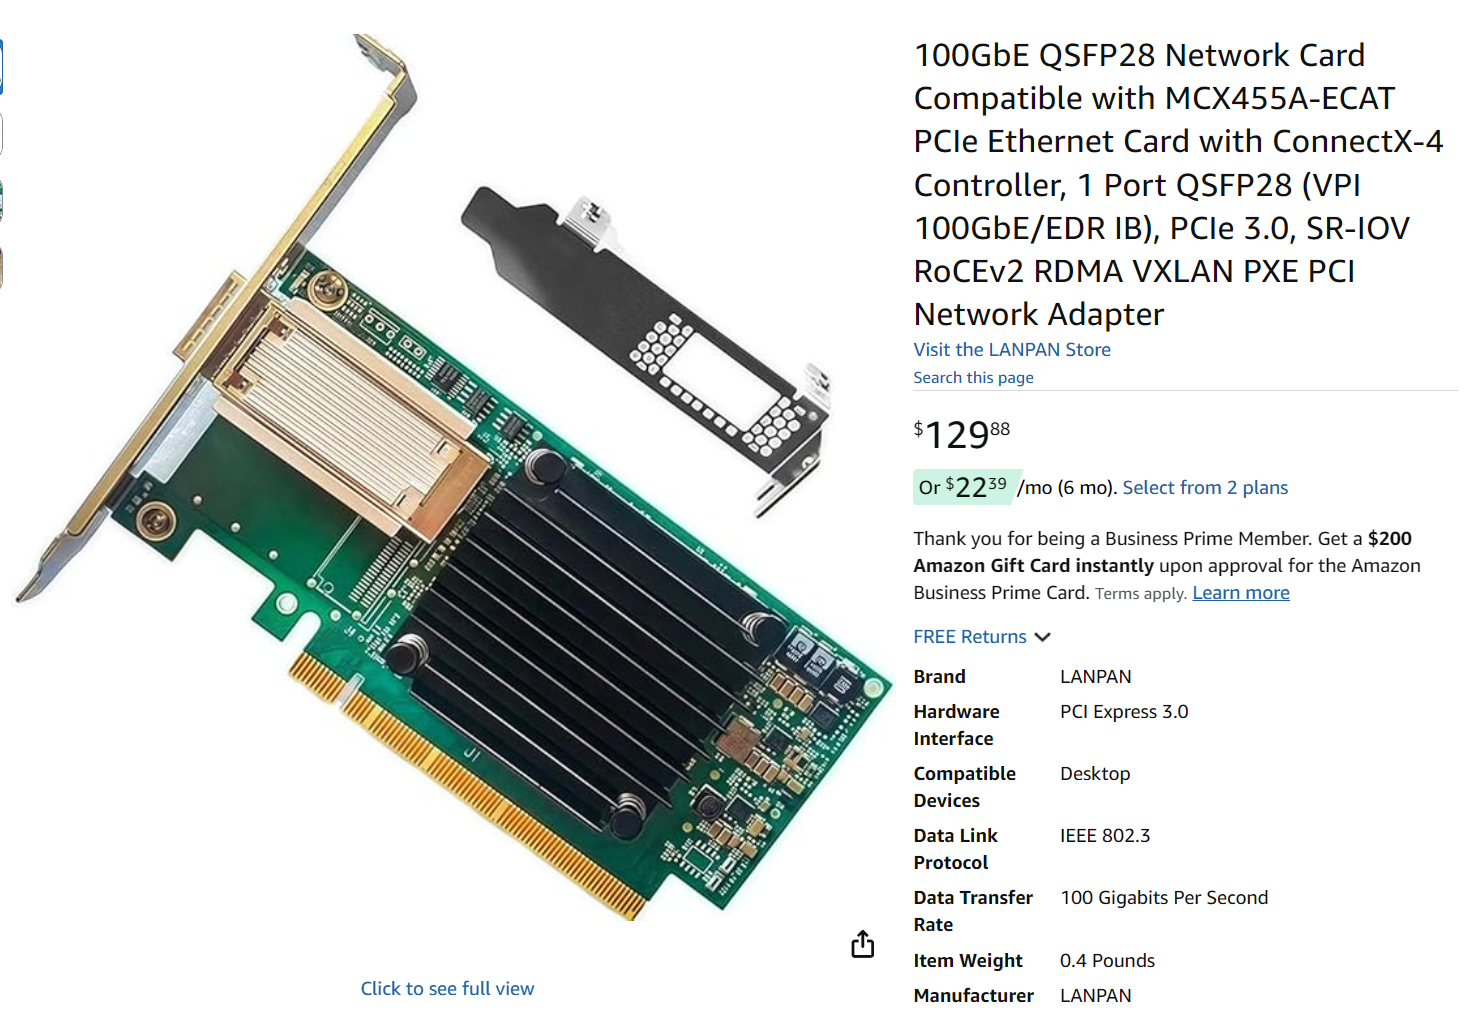
\includegraphics[width=\textwidth]{nic-lanpan-100gbe-amazon.png}
        \caption{LANPAN 100GbE QSFP28 Single Port -- \$129.88}
    \end{subfigure}
    \hfill
    \begin{subfigure}[b]{0.47\textwidth}
        \centering
        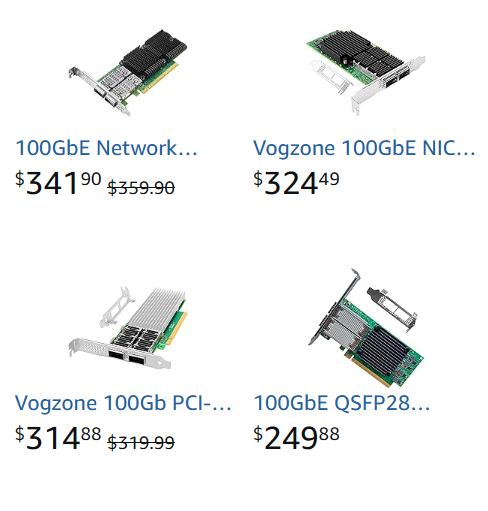
\includegraphics[width=\textwidth]{nic-100gbe-amazon-options.png}
        \caption{Various 100GbE options -- \$249--\$341}
    \end{subfigure}
    \caption{100GbE Network Card Options (Amazon)}
\end{figure}

\begin{figure}[H]
    \centering
    \begin{subfigure}[b]{0.47\textwidth}
        \centering
        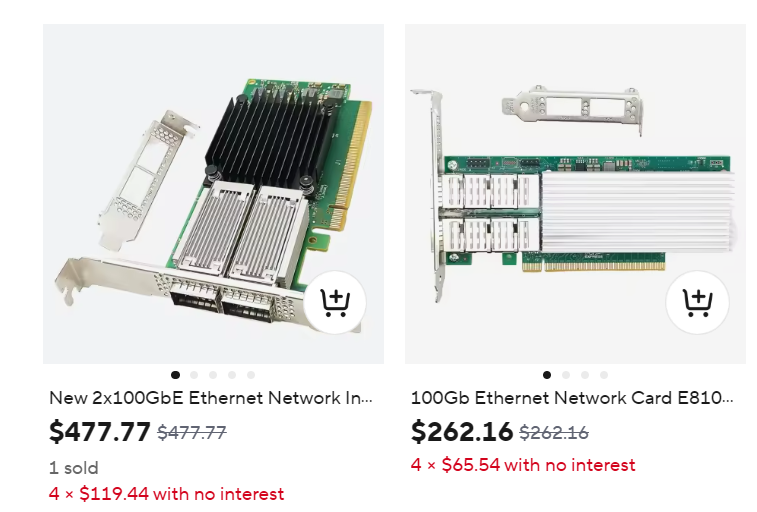
\includegraphics[width=\textwidth]{nic-dualport-100gbe-ebay.png}
        \caption{Dual-port 100GbE cards -- \$262--\$477}
    \end{subfigure}
    \hfill
    \begin{subfigure}[b]{0.47\textwidth}
        \centering
        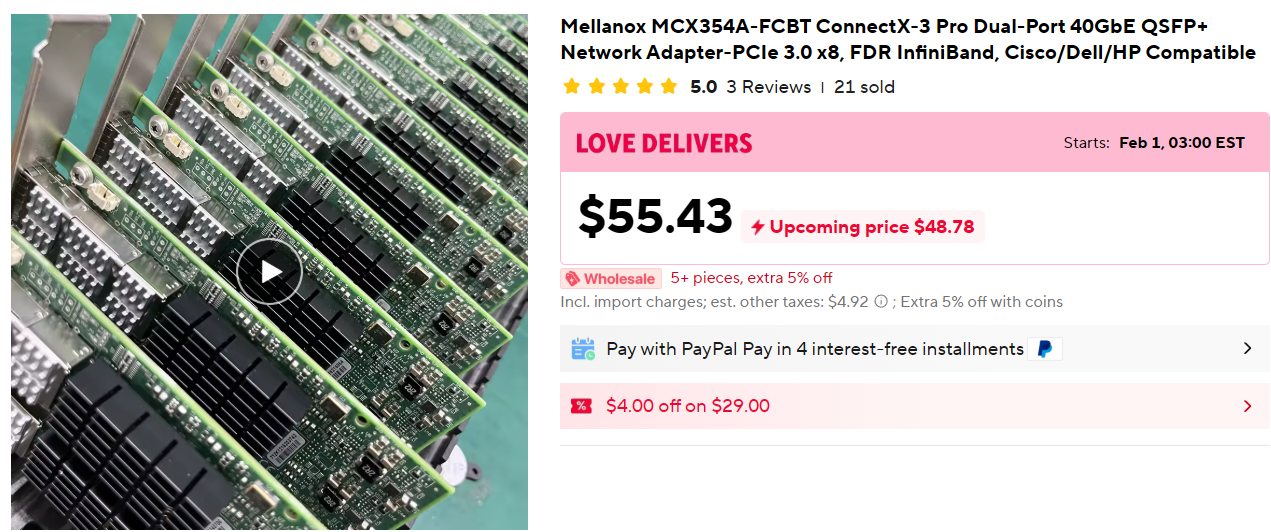
\includegraphics[width=\textwidth]{nic-mellanox-cx3-40gbe.png}
        \caption{Mellanox ConnectX-3 Pro 40GbE -- \$55.43}
    \end{subfigure}
    \caption{Additional Network Card Options (eBay)}
\end{figure}

\subsection{Hardware Purchases \& Price Analysis}

Strategic timing on hardware purchases saved significant money. For context on GPU pricing for LLM workloads, see \href{https://www.reddit.com/r/LocalLLaMA/comments/1p3d34y/inspired_by_a_recent_post_a_list_of_the_cheapest/}{this community-compiled list of cheapest VRAM options}. The Tesla V100 32GB originally launched at \href{https://www.microway.com/hpc-tech-tips/nvidia-tesla-v100-price-analysis/}{\$11,458 MSRP}---I paid \$626--\$669 each (94\% off).

\subsubsection{What I Purchased}

\begin{figure}[H]
    \centering
    \begin{subfigure}[b]{0.31\textwidth}
        \centering
        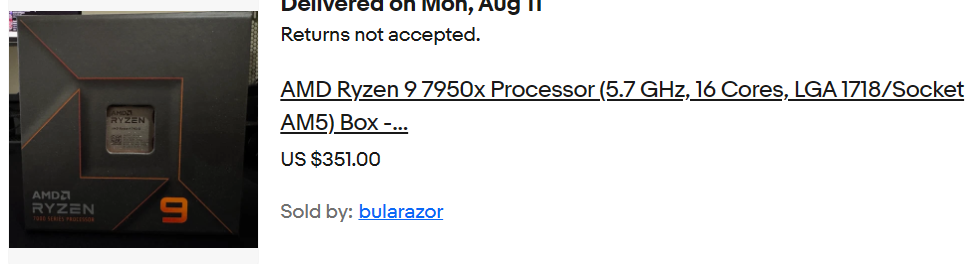
\includegraphics[width=\textwidth,height=3.5cm,keepaspectratio]{purchase-ryzen-7950x.png}
        \caption{Purchased: \$351 (Aug 2025)}
    \end{subfigure}
    \hfill
    \begin{subfigure}[b]{0.31\textwidth}
        \centering
        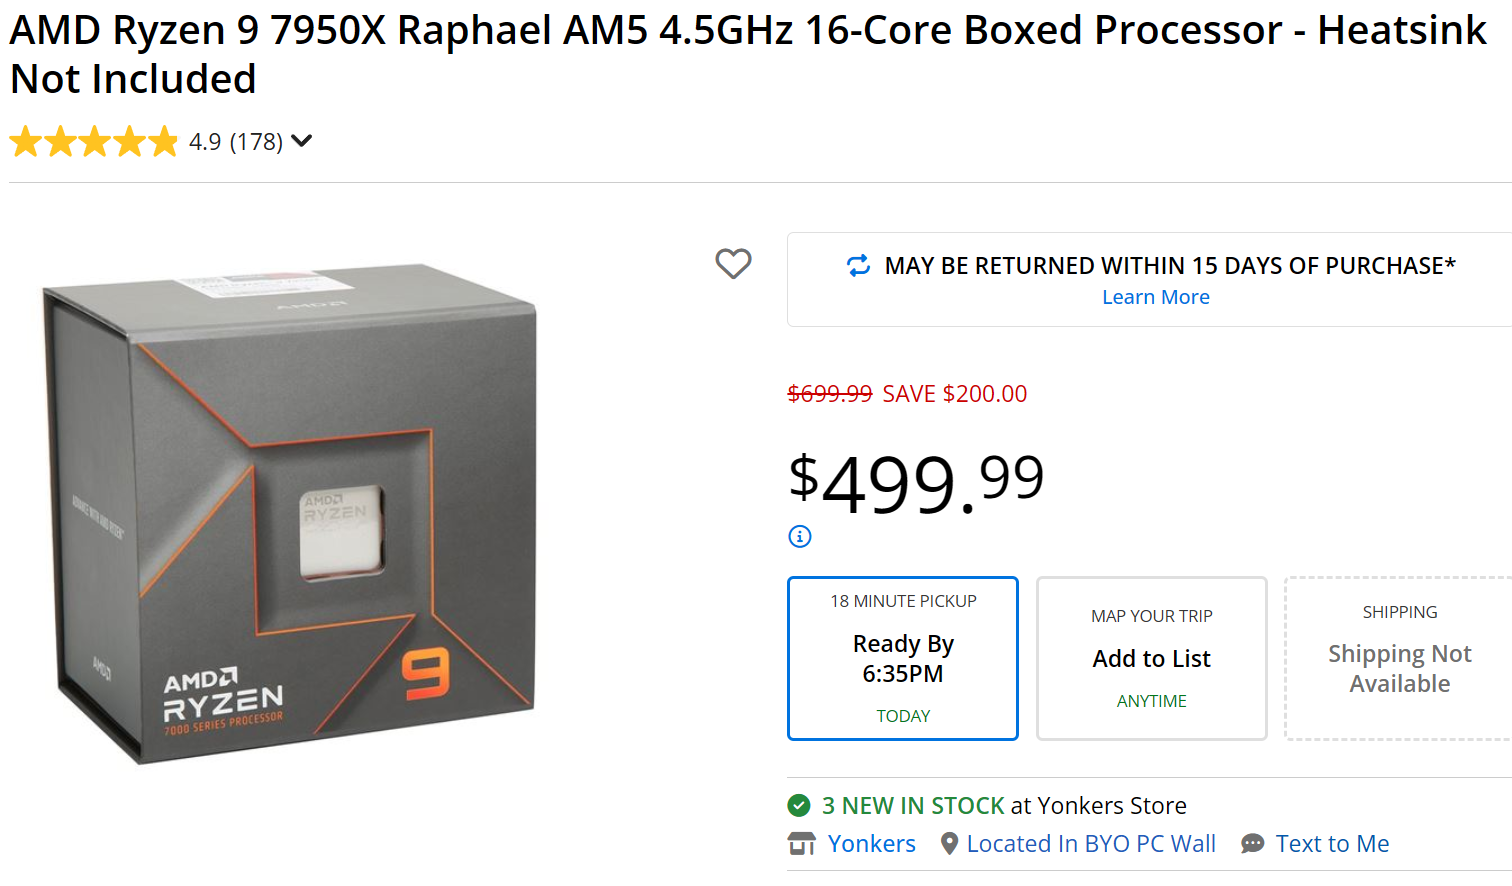
\includegraphics[width=\textwidth,height=3.5cm,keepaspectratio]{ryzen-7950x-current-price.png}
        \caption{Current: \$499 (Jan 2026)}
    \end{subfigure}
    \hfill
    \begin{subfigure}[b]{0.31\textwidth}
        \centering
        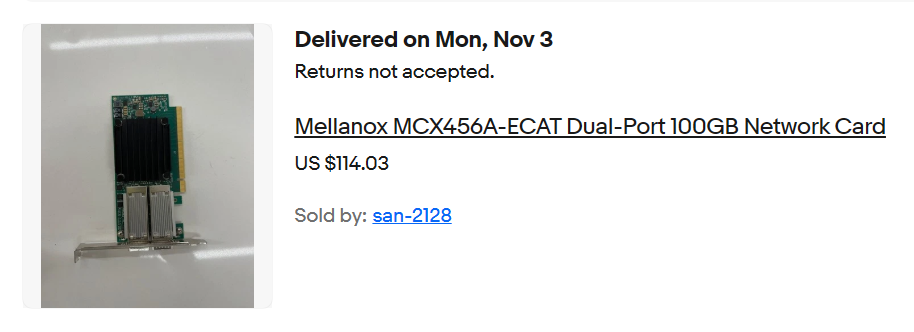
\includegraphics[width=\textwidth,height=3.5cm,keepaspectratio]{purchase-mellanox-mcx456a.png}
        \caption{Mellanox 100GbE: \$114}
    \end{subfigure}
    \caption{CPU and Network Card -- Saved \$148 on CPU alone}
\end{figure}

\begin{figure}[H]
    \centering
    \begin{subfigure}[b]{0.47\textwidth}
        \centering
        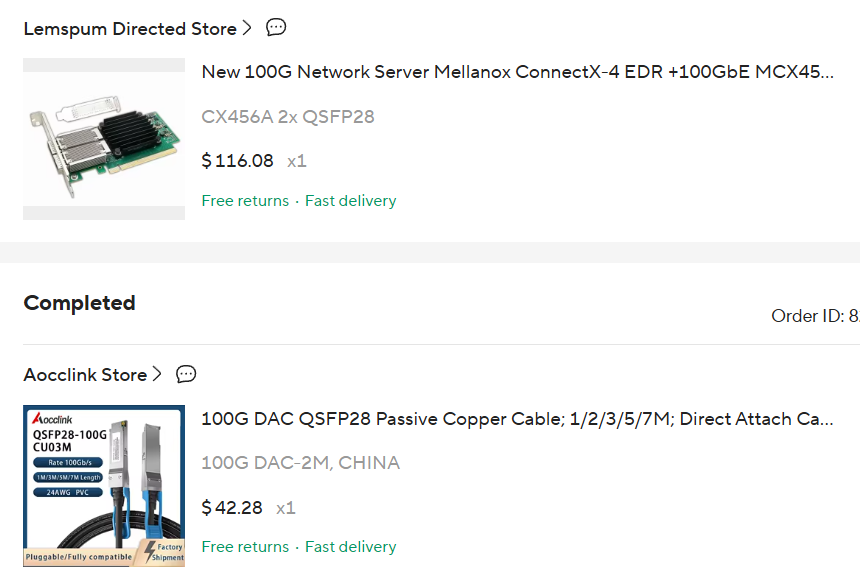
\includegraphics[width=\textwidth]{order-connectx4-dac.png}
        \caption{Mellanox ConnectX-4 + DAC Cable -- \$158 total}
    \end{subfigure}
    \hfill
    \begin{subfigure}[b]{0.47\textwidth}
        \centering
        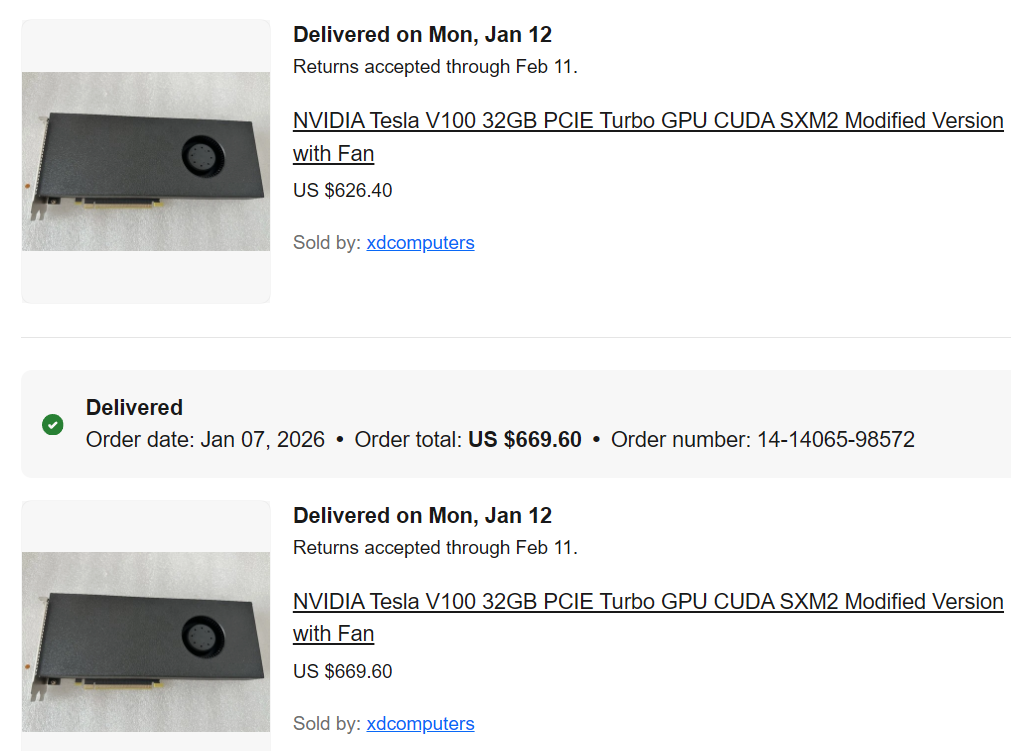
\includegraphics[width=\textwidth]{order-v100-gpus.png}
        \caption{2$\times$ Tesla V100 32GB SXM2 -- \$1,296 total}
    \end{subfigure}
    \caption{GPU and Additional Network Hardware Orders}
\end{figure}

\begin{figure}[H]
    \centering
    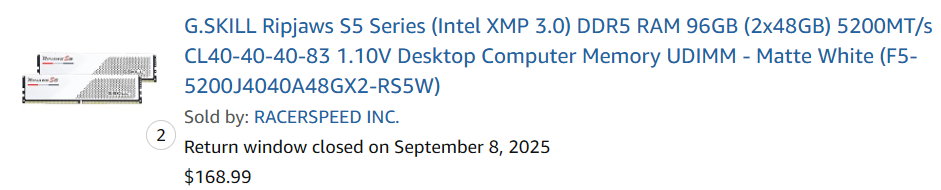
\includegraphics[width=0.6\textwidth]{ddr5-price-spike.png}
    \caption{DDR5 192GB (2$\times$96GB kits) -- \$337.98 total (Sep 2025, now \$2,000+)}
\end{figure}

\subsubsection{Current Market Prices (January 2026)}

\begin{figure}[H]
    \centering
    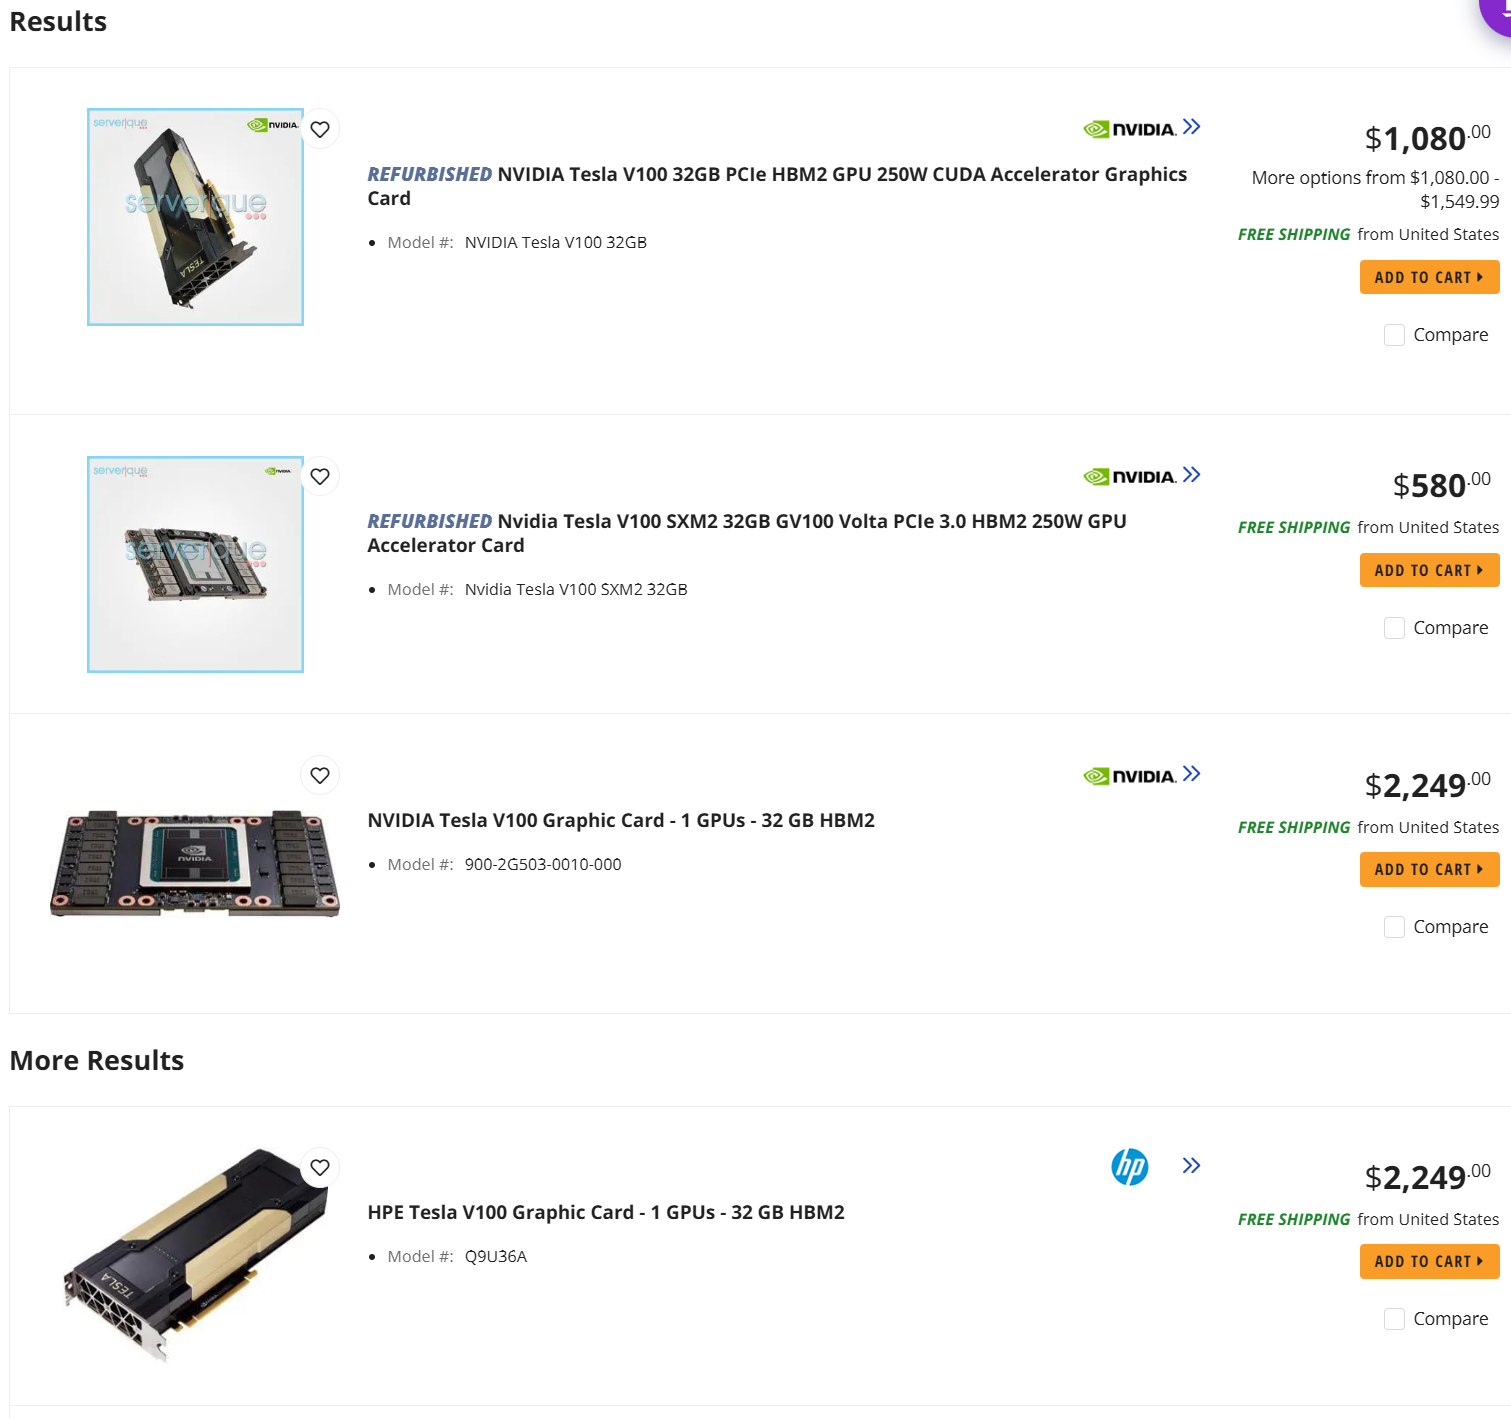
\includegraphics[width=0.75\textwidth]{v100-current-prices.png}
    \caption{V100 32GB prices today: \$580--\$2,249 (I paid \$626--\$669 each)}
\end{figure}

\begin{figure}[H]
    \centering
    \begin{subfigure}[b]{0.47\textwidth}
        \centering
        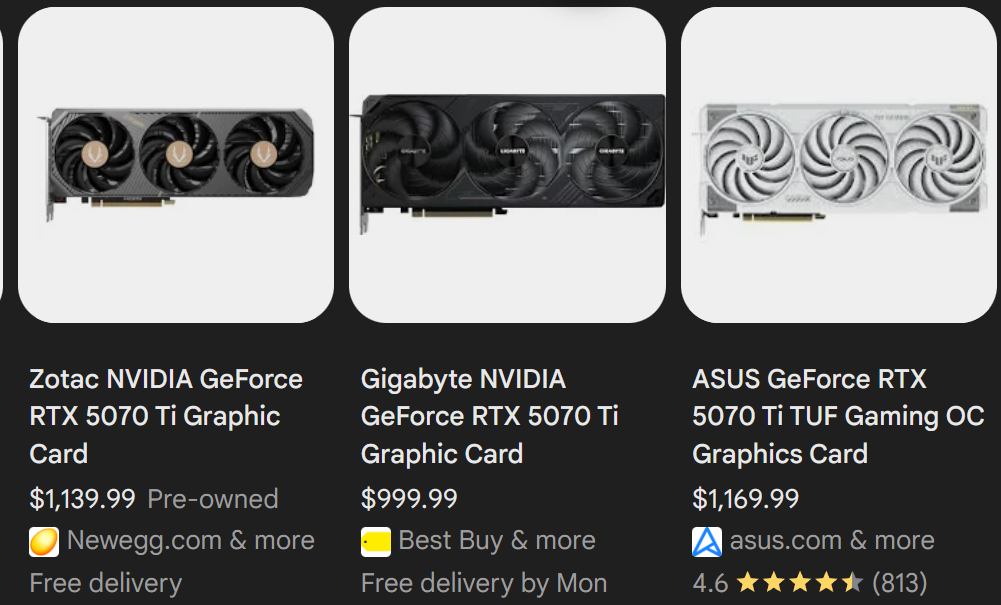
\includegraphics[width=\textwidth]{rtx5070ti-current-prices.png}
        \caption{RTX 5070 Ti current prices -- \$999--\$1,169}
    \end{subfigure}
    \hfill
    \begin{subfigure}[b]{0.47\textwidth}
        \centering
        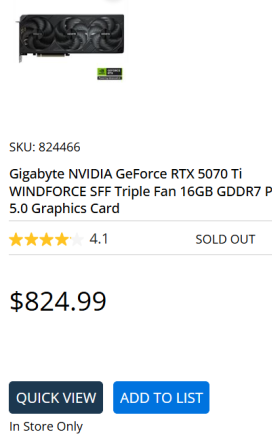
\includegraphics[width=\textwidth]{rtx5070ti-bestbuy-soldout.png}
        \caption{Gigabyte 5070 Ti -- \$824.99 (sold out)}
    \end{subfigure}
    \caption{Current RTX 5070 Ti Market Prices}
\end{figure}

\subsubsection{RAM Price Crisis}

DDR5 prices have exploded since late 2025 due to supply constraints and AI demand. I purchased 192GB (4$\times$48GB) of DDR5-5200 before the spike.

\begin{figure}[H]
    \centering
    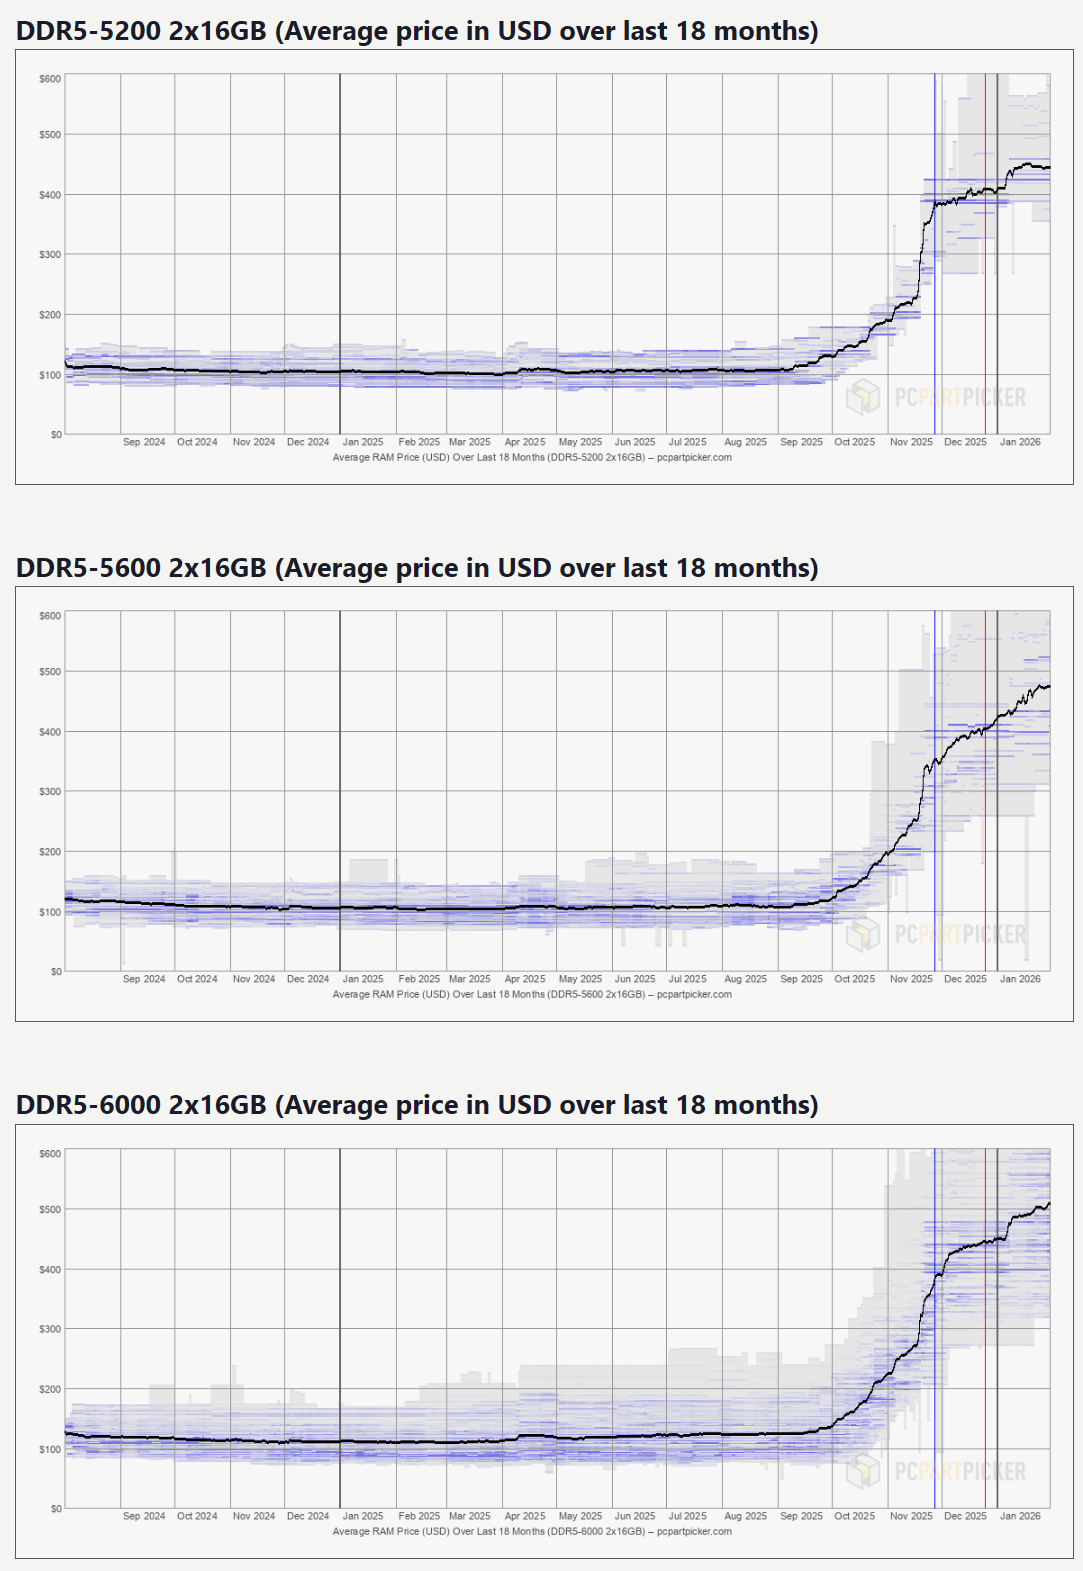
\includegraphics[width=0.75\textwidth,height=8cm,keepaspectratio]{ddr5-price-charts.png}
    \caption{DDR5 prices over 18 months -- stable at \$100 until Oct 2025, now \$400--\$500 (PCPartPicker)}
\end{figure}

\begin{figure}[H]
    \centering
    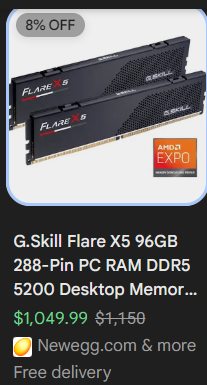
\includegraphics[width=0.25\textwidth]{ddr5-96gb-current-price.png}
    \caption{Current price: G.Skill 96GB DDR5-5200 kit -- \$1,049}
\end{figure}

\subsubsection{Inspiration}

\begin{figure}[H]
    \centering
    \begin{subfigure}[b]{0.47\textwidth}
        \centering
        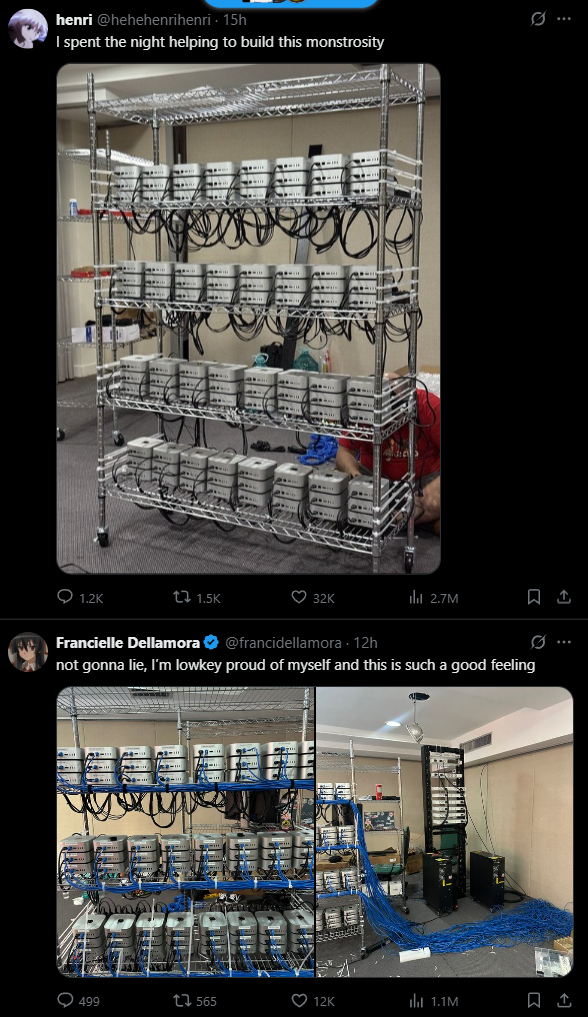
\includegraphics[width=\textwidth,height=4cm,keepaspectratio]{mac-mini-clusters.png}
        \caption{Community Mac Mini clusters}
    \end{subfigure}
    \hfill
    \begin{subfigure}[b]{0.47\textwidth}
        \centering
        \includegraphics[width=\textwidth,height=4cm,keepaspectratio]{homelab-open-frame.png}
        \caption{Open-frame homelab with storage arrays}
    \end{subfigure}
    \caption{Community builds for distributed inference}
\end{figure}

\subsection{Custom BIOS for Resizable BAR}

For my Homelabs, I had to flash a \href{https://github.com/ndg8743/x99-udp4-rebar}{custom BIOS} to enable Resizable BAR and 4G Decoding for the network card.

\begin{figure}[H]
    \centering
    \begin{subfigure}[b]{0.47\textwidth}
        \centering
        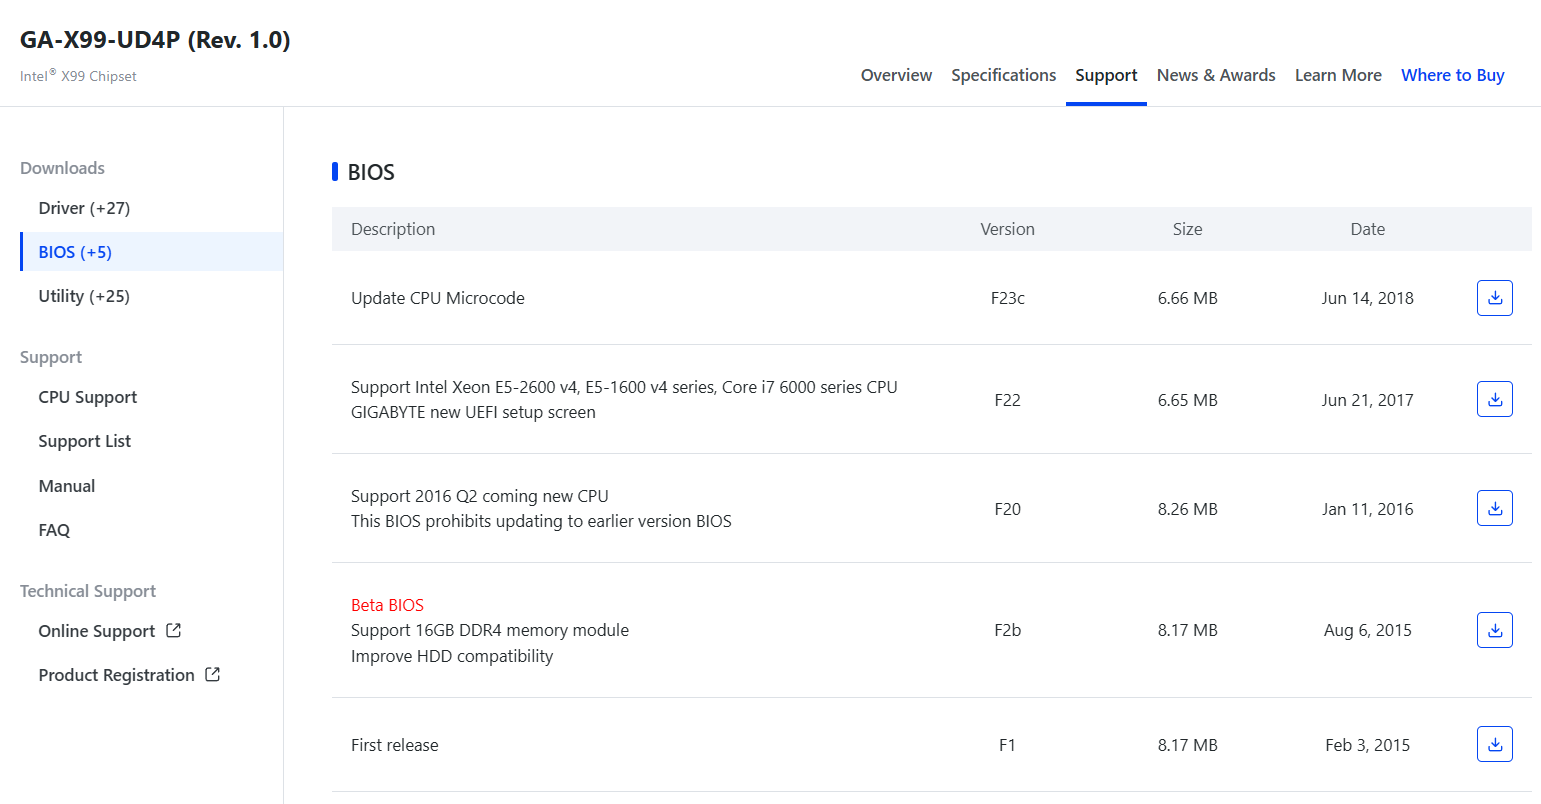
\includegraphics[width=\textwidth]{bios-official-versions.png}
        \caption{Official BIOS versions (F23c latest)}
    \end{subfigure}
    \hfill
    \begin{subfigure}[b]{0.47\textwidth}
        \centering
        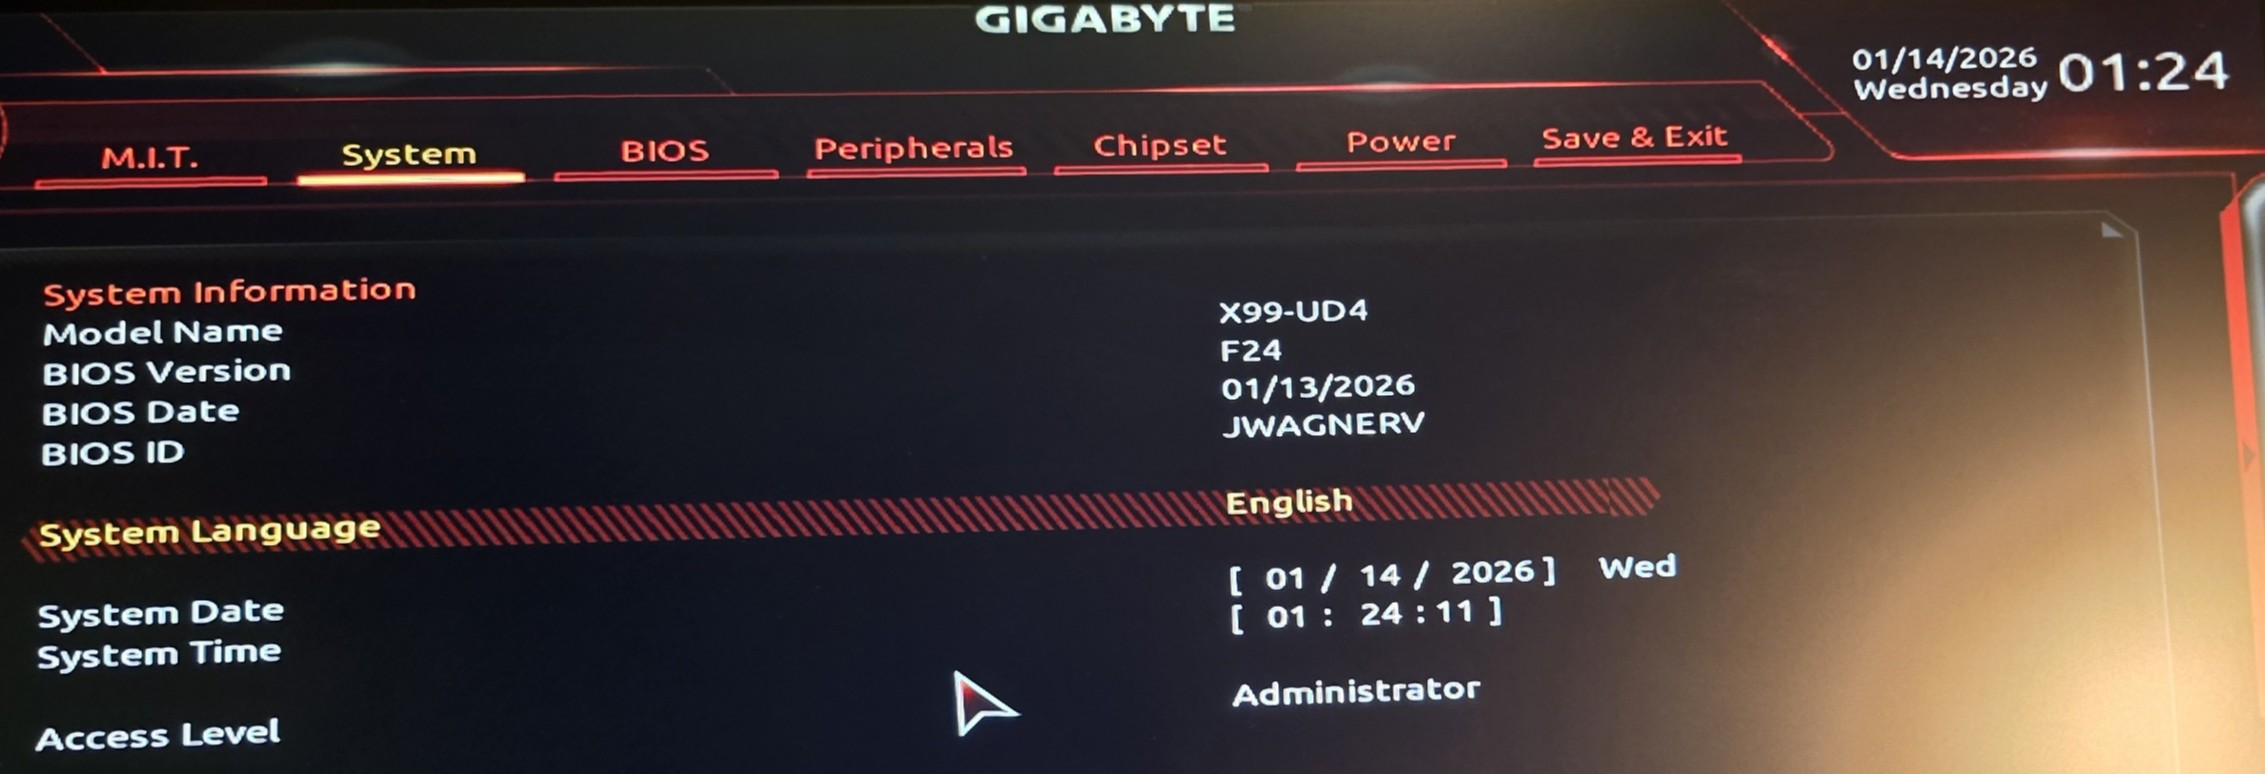
\includegraphics[width=\textwidth]{bios-custom-f24-rebar.jpg}
        \caption{Custom BIOS F24 with ReBAR support}
    \end{subfigure}
    \caption{GA-X99-UD4P BIOS -- Custom F24 adds Resizable BAR and 4G Decoding}
\end{figure}

\textit{Note: I still need to order a PCIe extender to fit between the 2 GPUs, or a higher wattage PSU for all GPUs to boot.}

\subsection{FPGA Options for DIY PCIe RDMA}

For the home towers (Chimera/Hydra/Cerberus), we can use RDMA on a DIY FPGA PCIe card or Mellanox cards (x16 slot gives $\sim$16 GB/s). When implementing custom FPGA solutions, security considerations are important---I enjoyed looking at the security optimizations in \href{https://ieeexplore.ieee.org/abstract/document/10682632}{Wafi's recent work from IEEE ISVLSI 2024}, which demonstrates deep learning approaches for detecting hardware trojans in FPGA bitstreams, achieving 93\% detection accuracy on Xilinx devices.

\begin{figure}[H]
    \centering
    \begin{subfigure}[b]{0.47\textwidth}
        \centering
        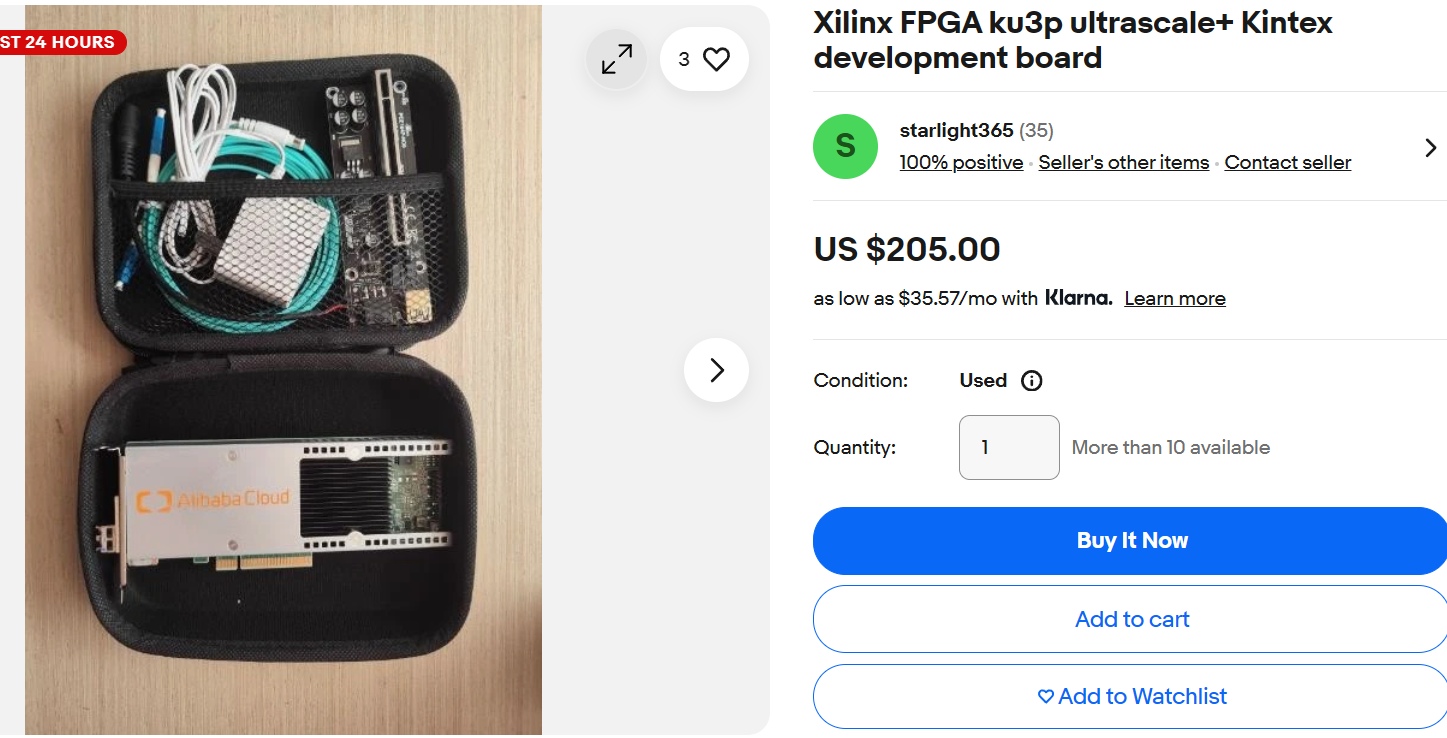
\includegraphics[width=\textwidth]{fpga-xilinx-ku3p-devboard.png}
        \caption{Xilinx FPGA KU3P UltraScale+ Kintex Dev Board -- \$205}
    \end{subfigure}
    \hfill
    \begin{subfigure}[b]{0.47\textwidth}
        \centering
        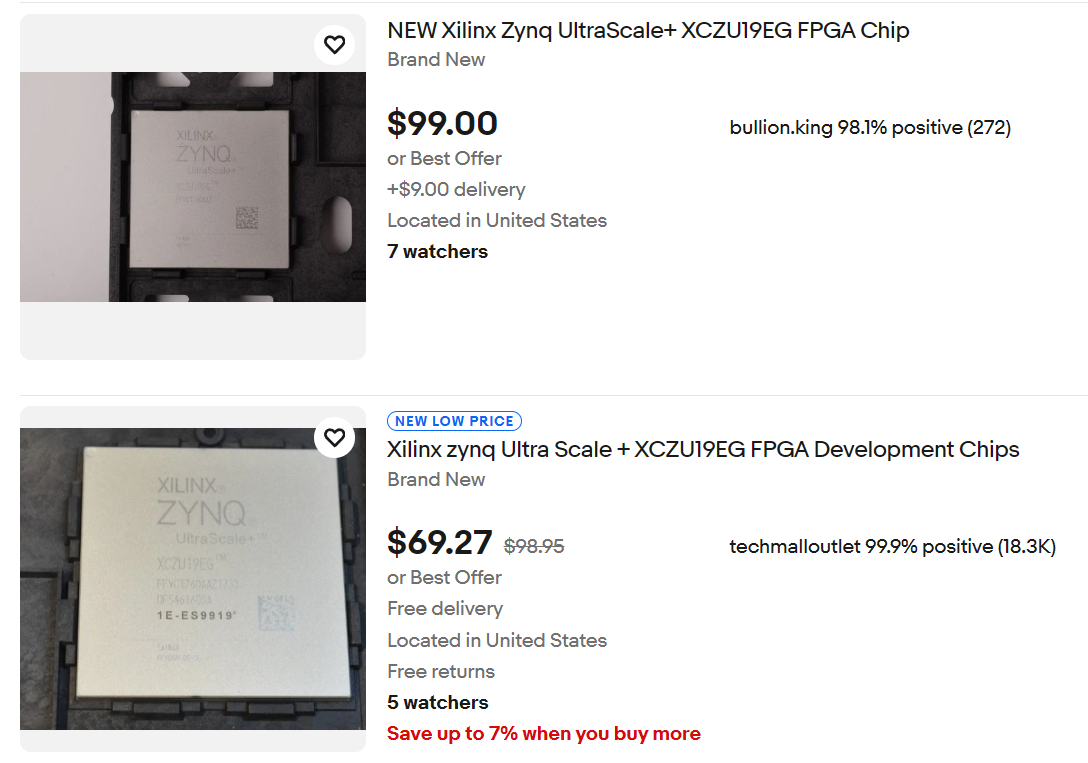
\includegraphics[width=\textwidth]{fpga-xilinx-zynq-chips.png}
        \caption{Xilinx Zynq UltraScale+ FPGA Chips -- \$69--\$99}
    \end{subfigure}
    \caption{FPGA Options for Custom RDMA Implementation}
\end{figure}

\subsection{Current Server Infrastructure}

My home setup consists of two towers with a combined 32 cores, 320GB RAM, and 100Gbit networking:

\textbf{Tower 1 (Windows):} Ryzen 9 7950X (16c/32t), 192GB DDR5-5200, RTX 5070 Ti (16GB GDDR7), 2TB Gen5 NVMe, 40TB+ HDD raw storage, 100GbE networking.

\textbf{Tower 2 (Proxmox):} Gigabyte X99 UD4P, Xeon E5-2697A v4 (16c/32t), 128GB DDR4 2133 ECC, 2$\times$ Tesla V100 32GB (needs PCIe extender to fit between GPUs or higher wattage PSU), 1TB Crucial NVMe, 2TB Seagate HDD, NZXT H440, 750W Bronze PSU, 100GbE networking.

\begin{figure}[H]
    \centering
    \begin{subfigure}[b]{0.47\textwidth}
        \centering
        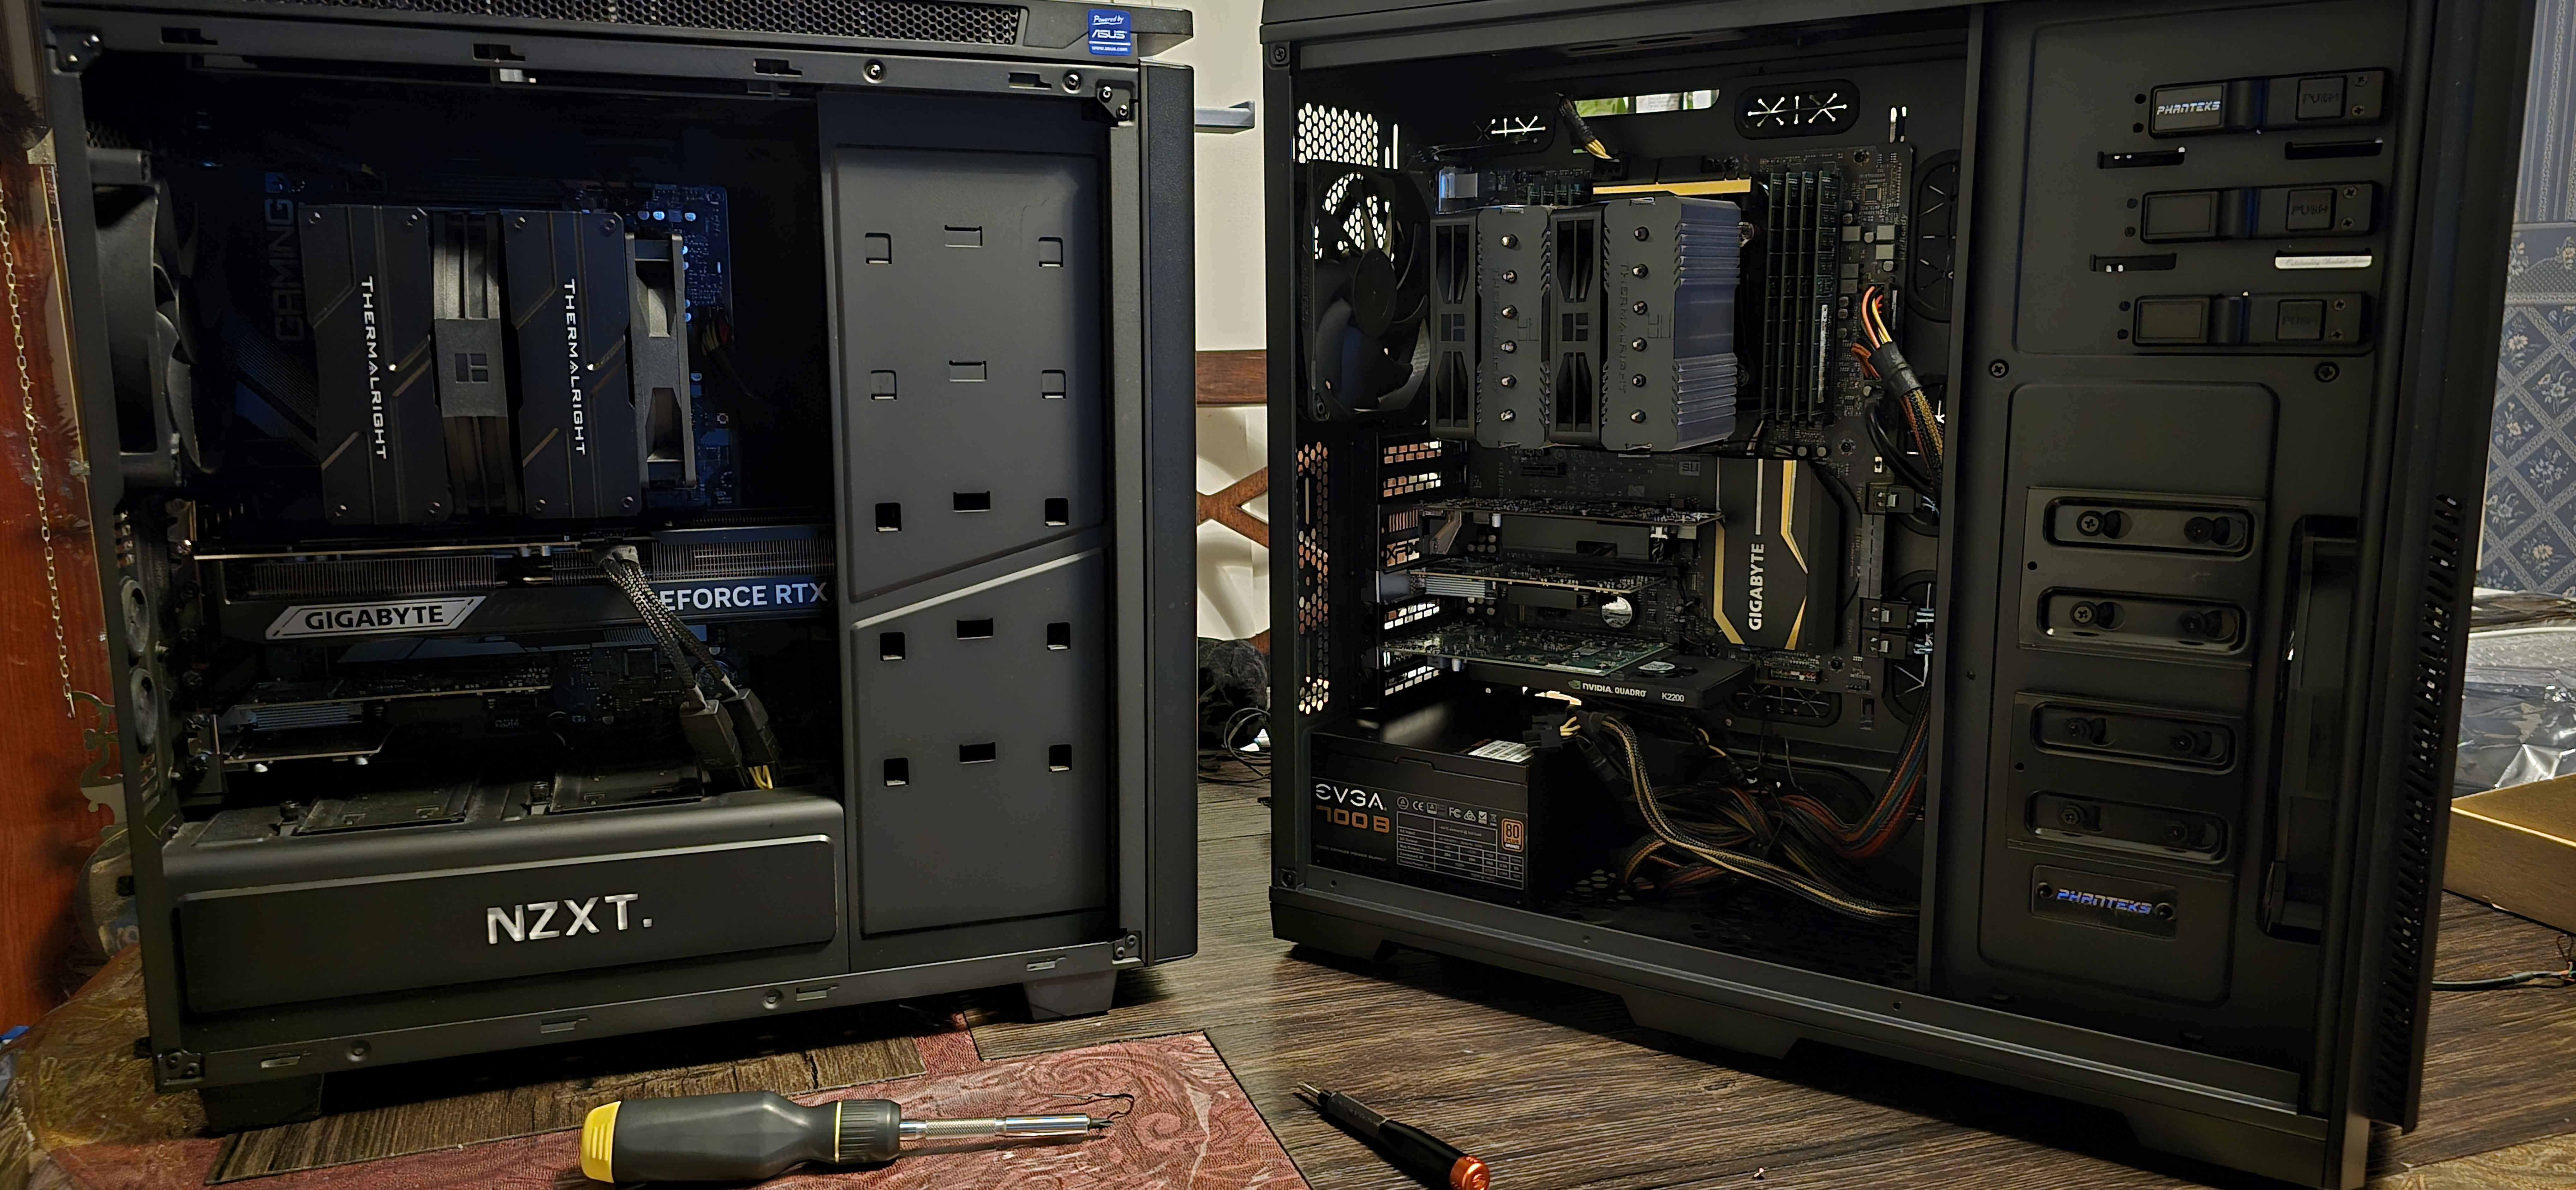
\includegraphics[width=\textwidth]{towers-initial-setup.jpg}
        \caption{Tower 1 (left) and Tower 2 (right) -- Initial setup}
    \end{subfigure}
    \hfill
    \begin{subfigure}[b]{0.47\textwidth}
        \centering
        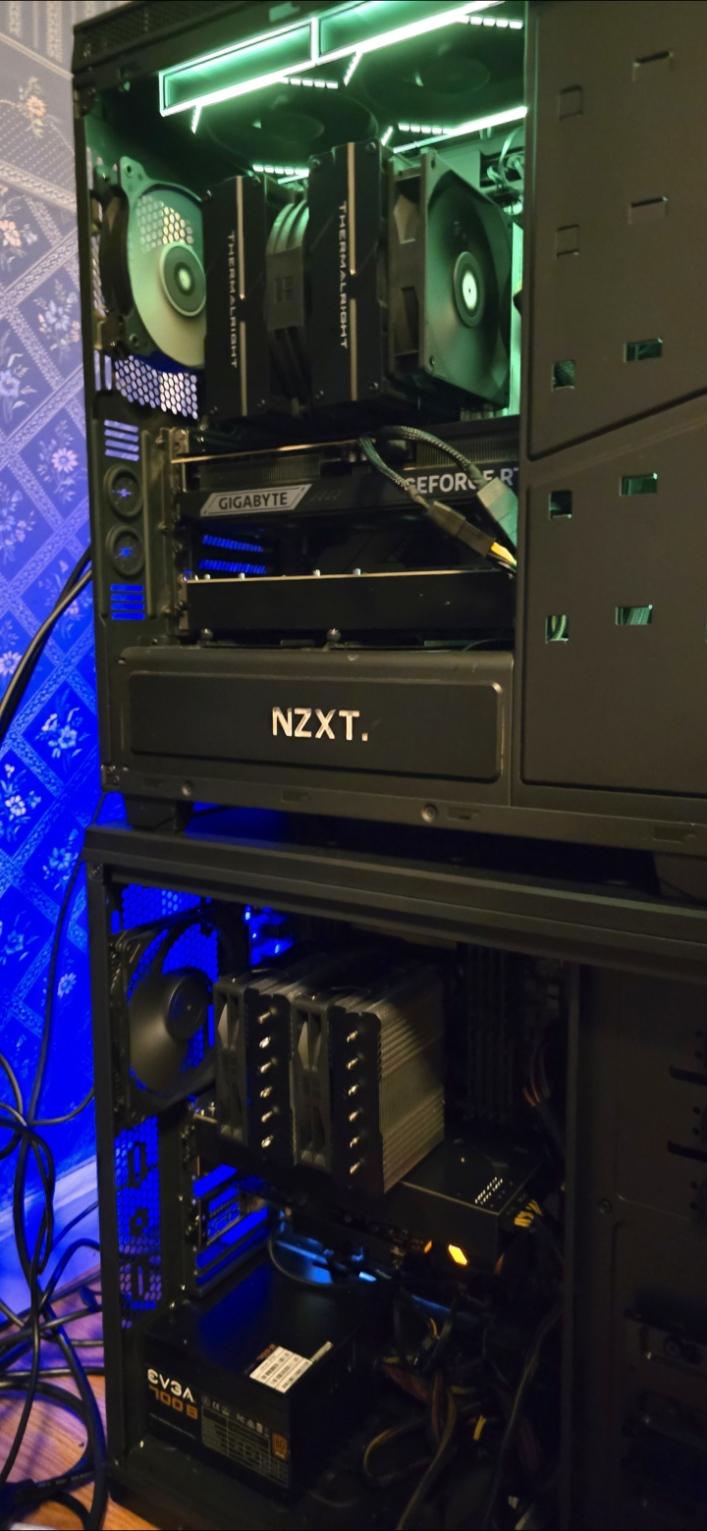
\includegraphics[width=\textwidth,height=4cm,keepaspectratio]{towers-stacked.jpg}
        \caption{Stacked configuration -- Tower 1 (top) and Tower 2 (bottom)}
    \end{subfigure}
    \caption{Home Lab -- The Two Main Towers}
\end{figure}

\begin{figure}[H]
    \centering
    \begin{subfigure}[b]{0.47\textwidth}
        \centering
        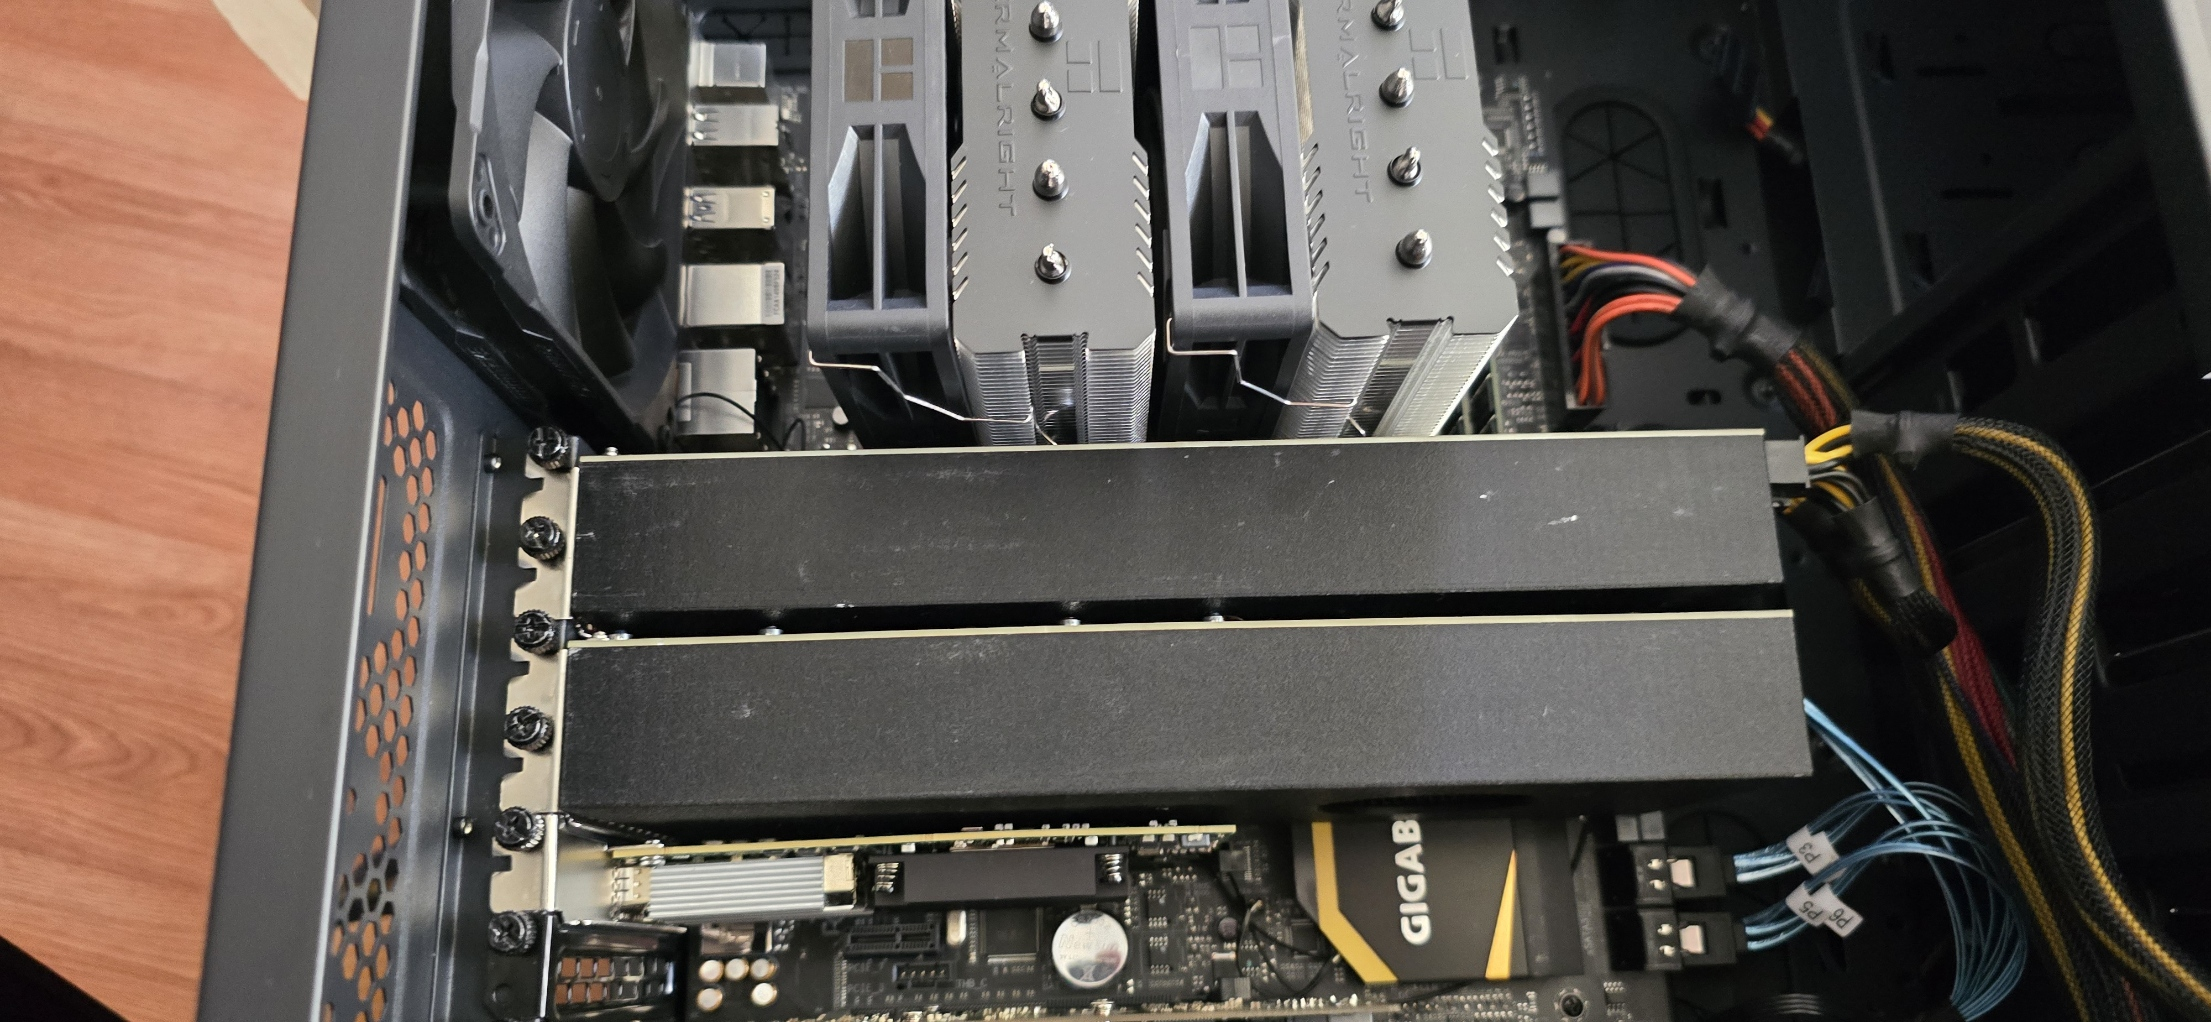
\includegraphics[width=\textwidth]{v100-gpus-installed.jpg}
        \caption{V100 GPUs installed in Tower 2}
    \end{subfigure}
    \hfill
    \begin{subfigure}[b]{0.47\textwidth}
        \centering
        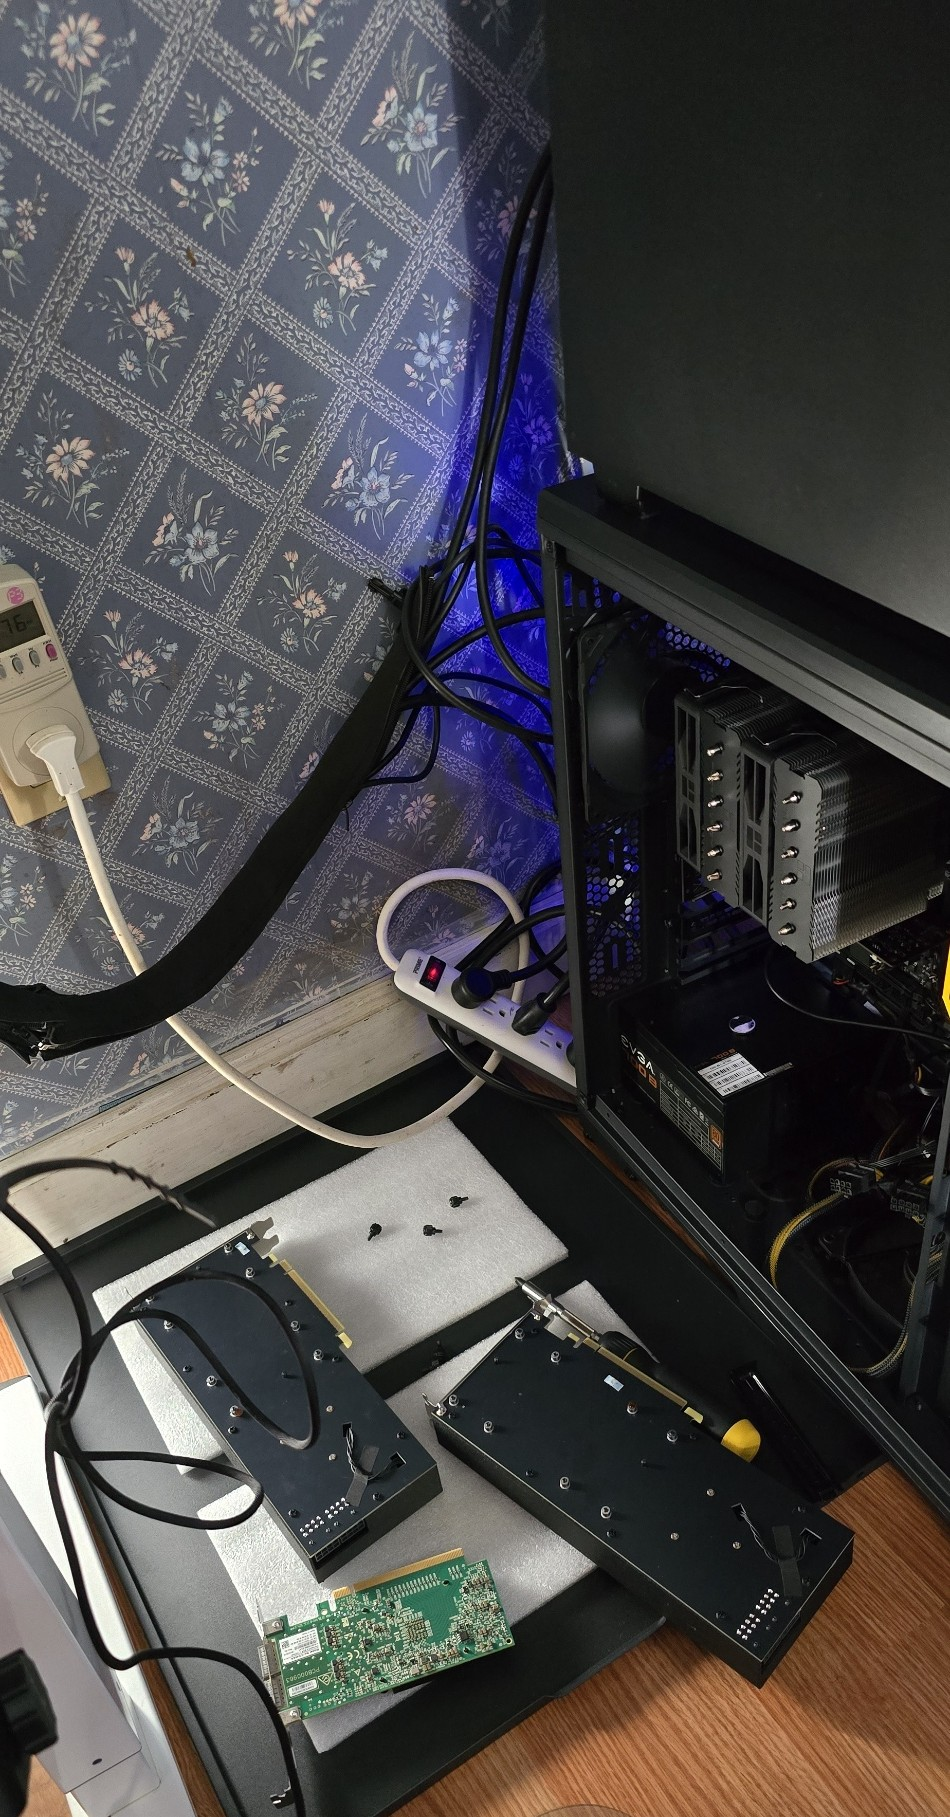
\includegraphics[width=\textwidth,height=4cm,keepaspectratio]{hardware-staging-v100s.jpg}
        \caption{Hardware staging -- V100s and network card}
    \end{subfigure}
    \caption{GPU Installation Progress}
\end{figure}

\begin{figure}[H]
    \centering
    \begin{subfigure}[b]{0.47\textwidth}
        \centering
        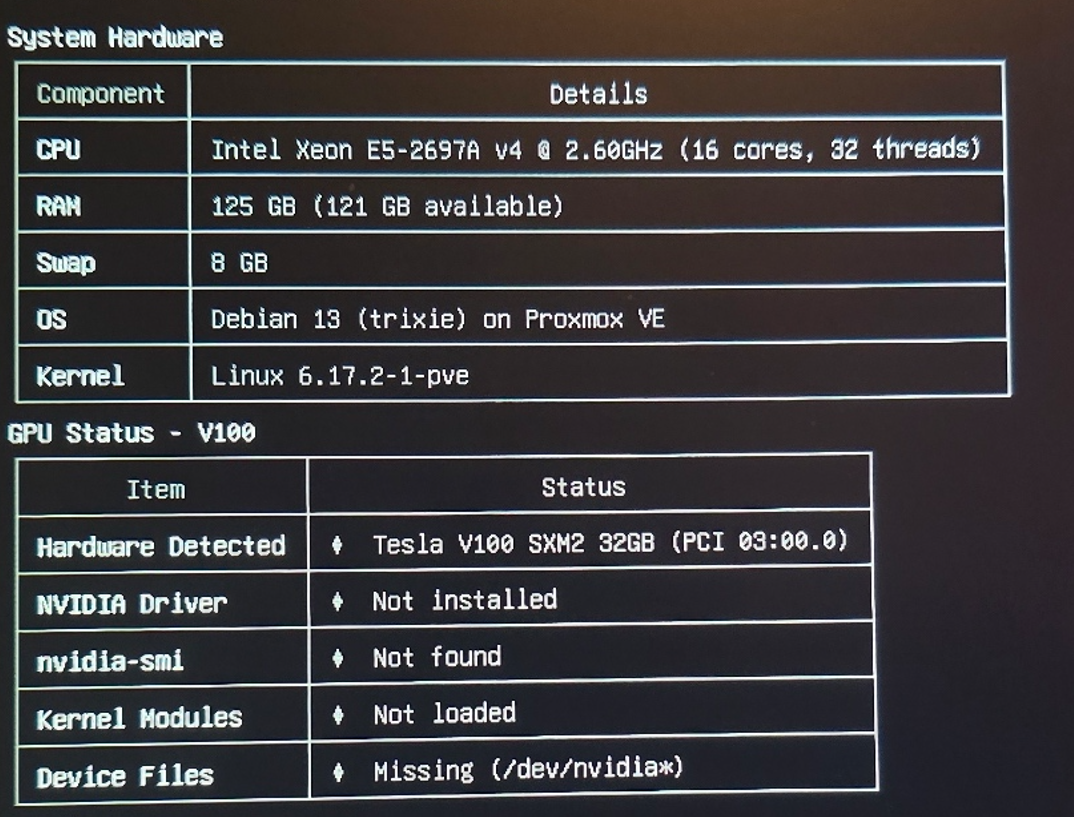
\includegraphics[width=\textwidth]{specs-proxmox-server.png}
        \caption{Tower 2: Xeon E5-2697A v4, 125GB RAM, V100 32GB}
    \end{subfigure}
    \hfill
    \begin{subfigure}[b]{0.47\textwidth}
        \centering
        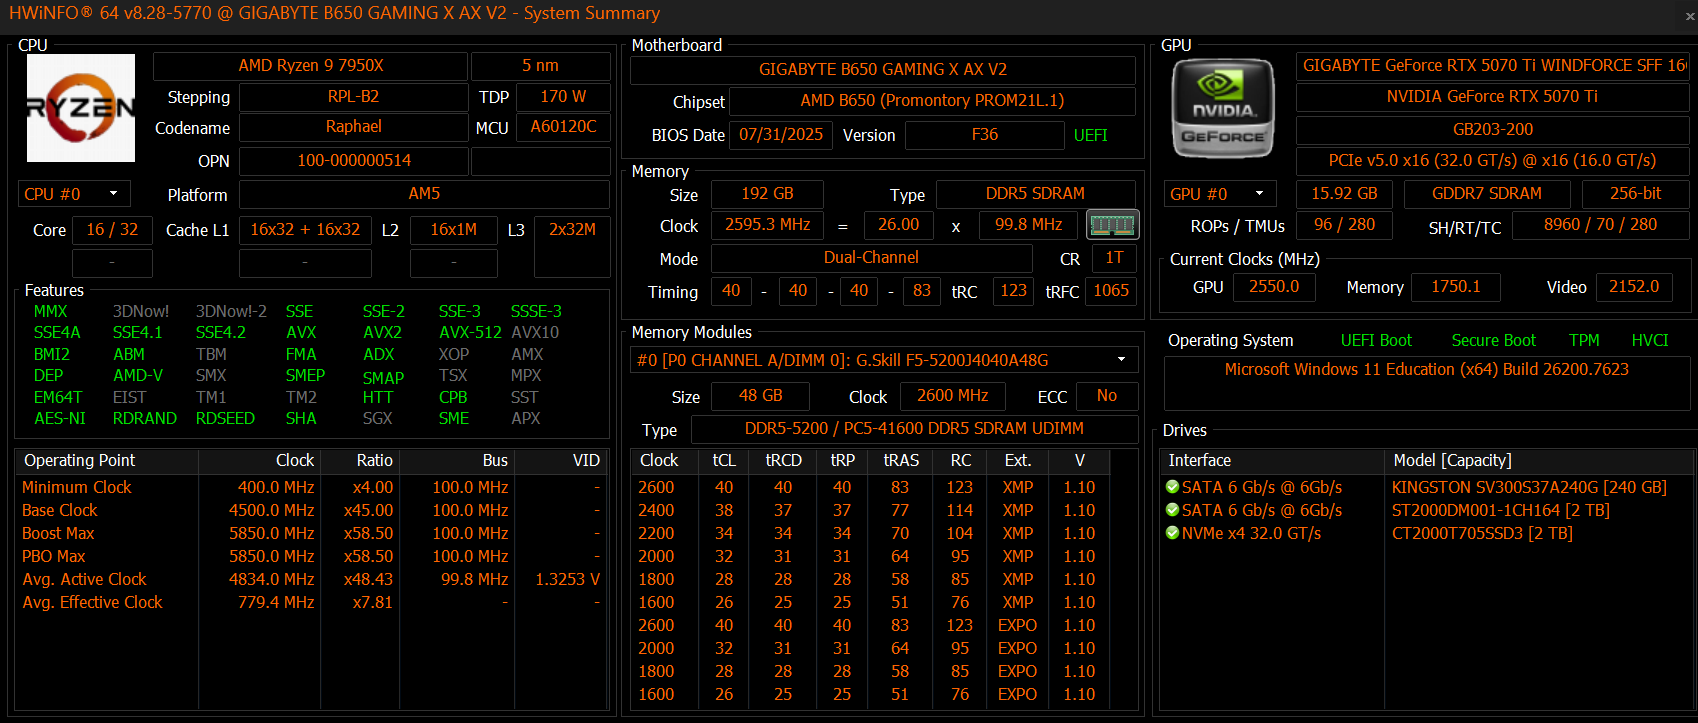
\includegraphics[width=\textwidth]{specs-workstation-hwinfo.png}
        \caption{Tower 1: Ryzen 9 7950X, 192GB RAM, RTX 5070 Ti}
    \end{subfigure}
    \caption{System Specifications}
\end{figure}

\subsection{Cost Analysis: Homelab vs Commercial Solutions}

\begin{table}[H]
\centering
\small
\begin{tabular}{@{}lrrr@{}}
\toprule
\textbf{Component} & \textbf{My Cost} & \textbf{MSRP/Current} & \textbf{Savings} \\
\midrule
\multicolumn{4}{@{}l@{}}{\textit{Tower 1 (Windows/Daily):}} \\
Ryzen 9 7950X & \$351 & \$499 & 30\% \\
192GB DDR5-5200 (4$\times$48GB) & \$338 & \$3,000+ & 89\% \\
RTX 5070 Ti 16GB & \$825 & \$825 & 0\% \\
\midrule
\multicolumn{4}{@{}l@{}}{\textit{Tower 2 (Proxmox/X99):}} \\
Gigabyte X99 UD4P + Xeon E5-2697A v4 & $\sim$\$300 & \$2,000+ & 85\% \\
128GB DDR4 2133 ECC & \$0 (free) & \$400+ & 100\% \\
2$\times$ Tesla V100 32GB & \$1,296 & \$22,916 & 94\% \\
NZXT H440 + 750W PSU + Cooler & $\sim$\$150 & \$300 & 50\% \\
\midrule
\multicolumn{4}{@{}l@{}}{\textit{Networking:}} \\
Mellanox 100GbE (2 cards + DAC) & \$272 & \$800+ & 66\% \\
\midrule
\textbf{Total Compute Hardware} & \textbf{$\sim$\$3,532} & \textbf{\$30,000+} & \textbf{88\%} \\
\bottomrule
\end{tabular}
\caption{Hardware Cost Breakdown}
\end{table}

\begin{table}[H]
\centering
\small
\begin{tabular}{@{}lrrrr@{}}
\toprule
\textbf{Solution} & \textbf{Cost} & \textbf{VRAM} & \textbf{Est. tok/s (70B)} & \textbf{\$/tok/s} \\
\midrule
My Homelab (2$\times$V100 + 5070 Ti) & \$3,532 & 80GB & $\sim$18 & \$196 \\
NVIDIA DGX A100 & \$199,000 & 640GB & $\sim$150 & \$1,327 \\
AWS p4d.24xlarge (1yr) & \$285,000 & 320GB & $\sim$80 & \$3,563 \\
Lambda Labs (1yr) & \$87,600 & 80GB & $\sim$20 & \$4,380 \\
Mac Studio M2 Ultra & \$4,000 & 192GB & $\sim$8 & \$500 \\
\bottomrule
\end{tabular}
\caption{Cost Efficiency Comparison -- Lower \$/tok/s = Better Value}
\end{table}

\begin{figure}[H]
    \centering
    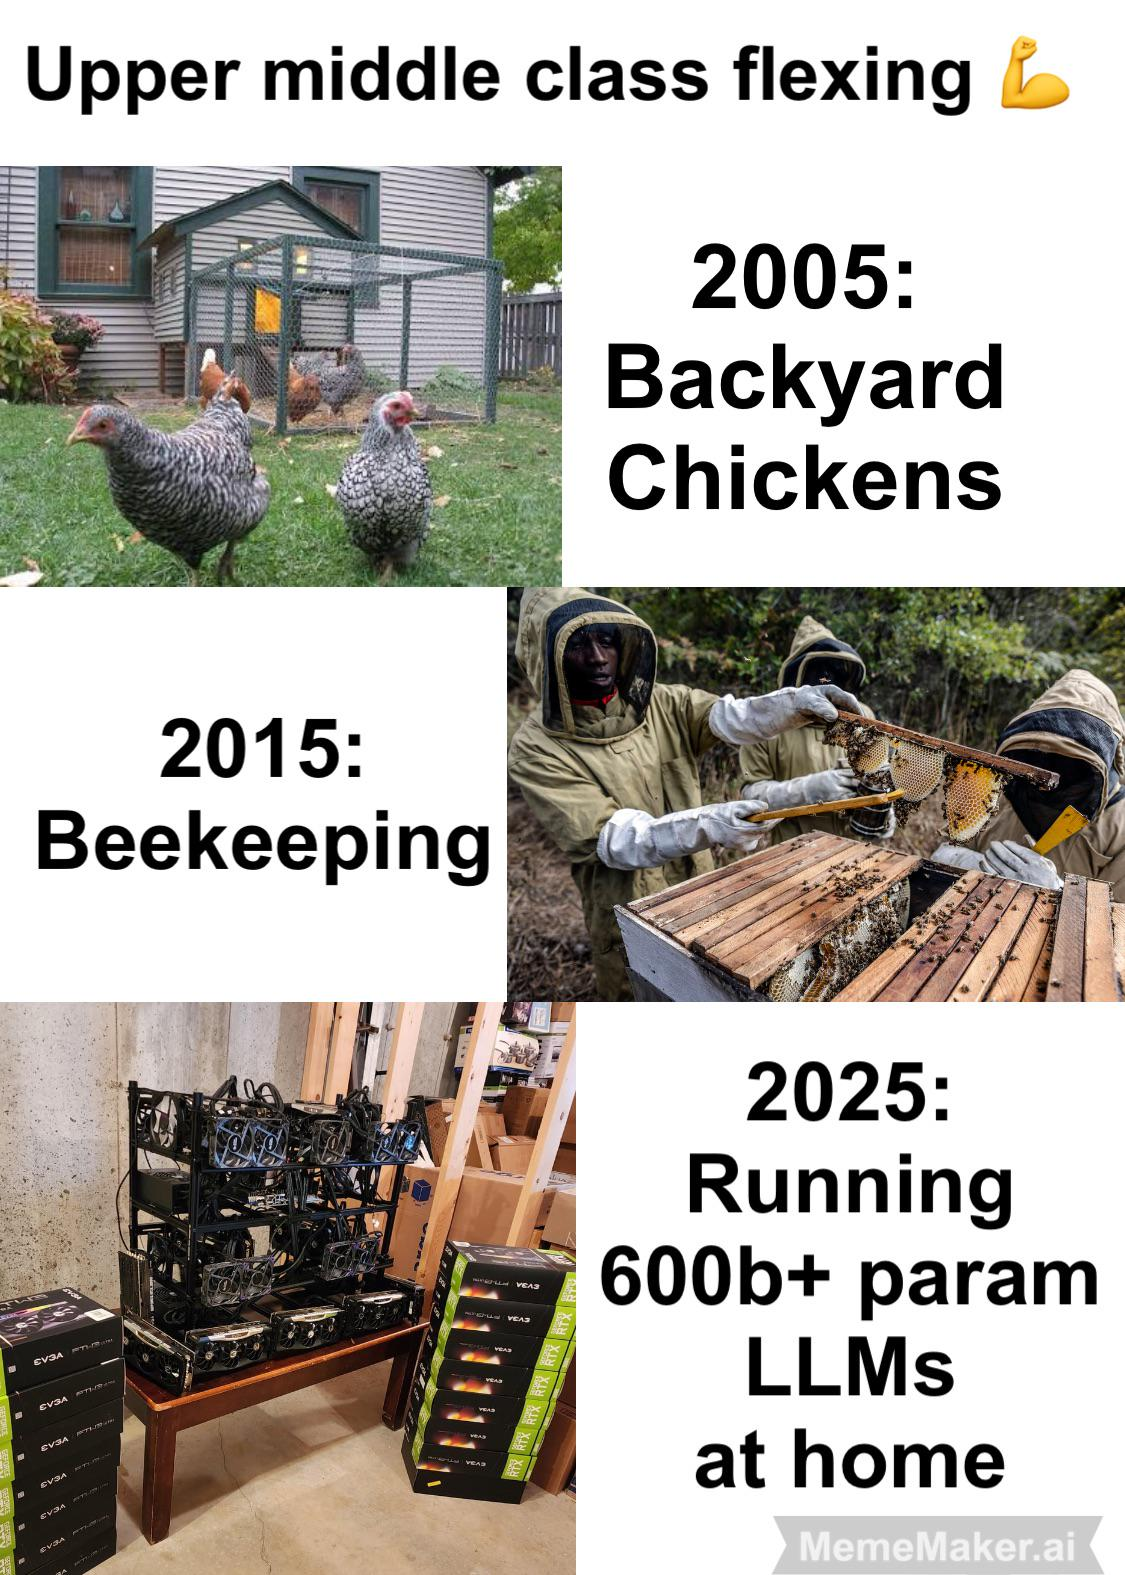
\includegraphics[width=0.35\textwidth]{meme-homelab-flexing.jpg}
\end{figure}

\end{document}
